\section{Partitionnement \'etendu: Choisir le but de l'installation}
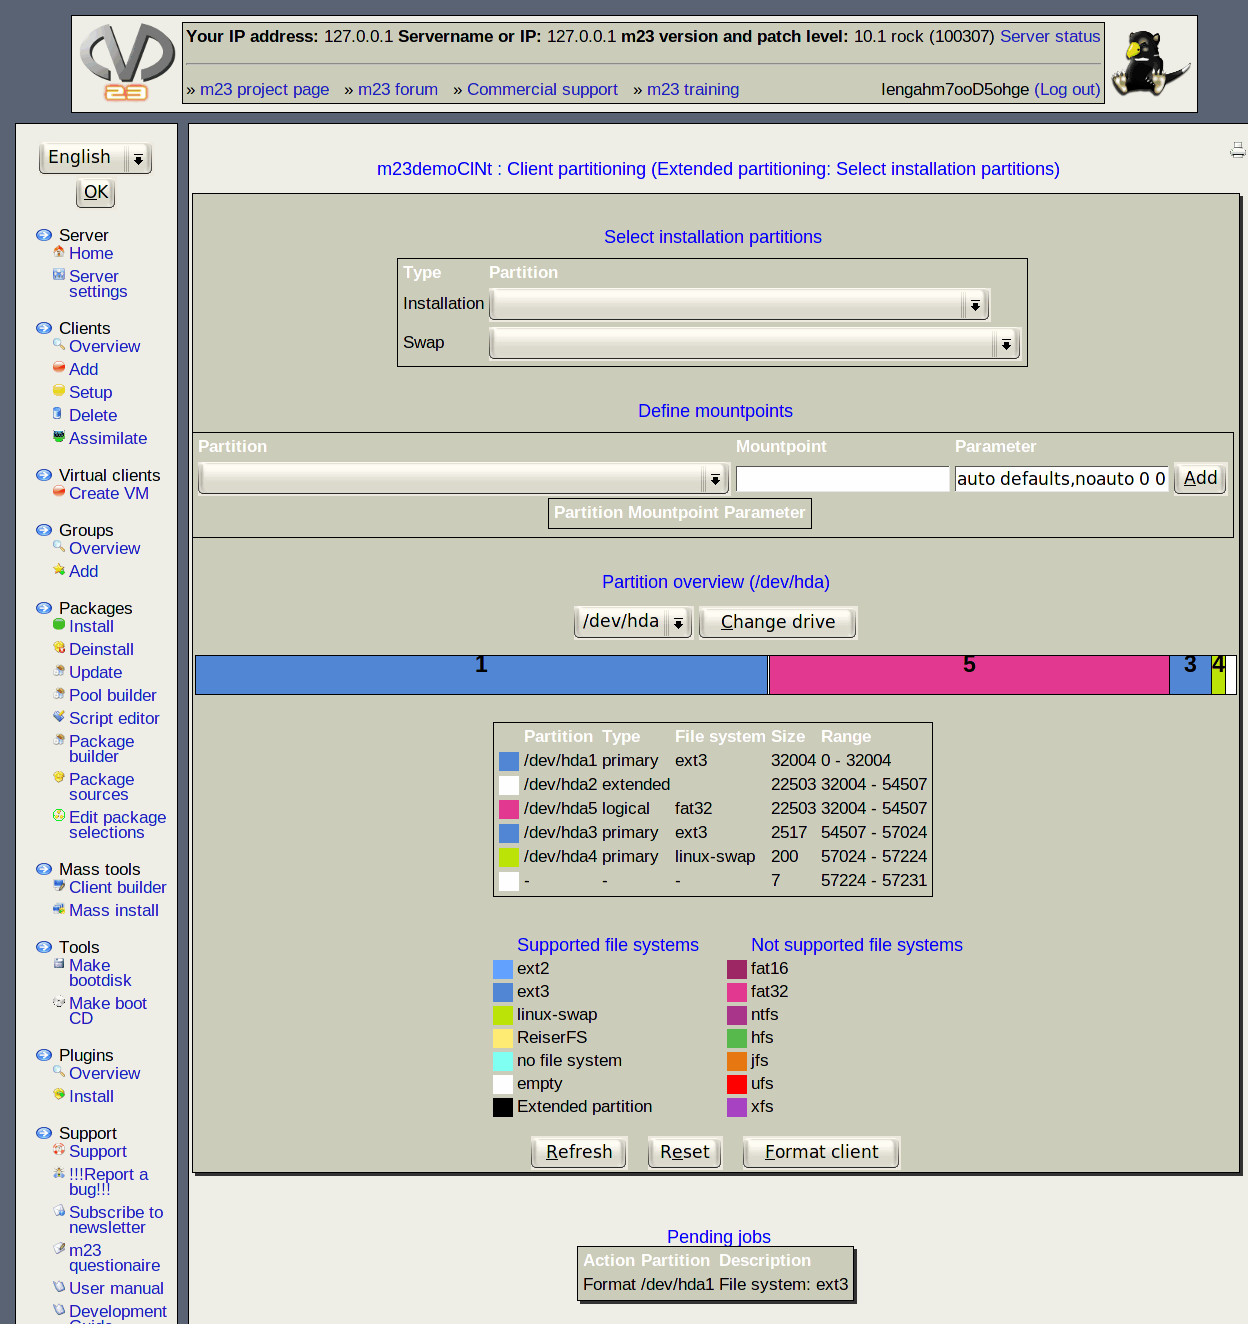
\includegraphics[scale=0.4]{/mdk/doc/manual/screenshots/fr/fdisk-extended3.png} \\
Choisissez deux partitions que vous voudriez utiliser pour l'installation - la premi\`ere pour l'installation du syst\`eme d'exploitation et la deuxi\`eme comme swap/permutation.\\
\subsection{Proc\'ed\'e \'etape par \'etape:}
\begin{enumerate}
\item S\'electionnez les partitions que vous voulez utiliser pour l'installation et comme swap.\\
\item Si vous avez besoin de points de montage additionels, vous pouvez les cr\'eer chez \textit{$\ll$Definer les points de montage$\gg$}. Entrez la partition, le point de montage et les param\`etres n\'ecessaires pour le montage et ensuite, cliquez sur \textit{$\ll$Ajouter$\gg$}. Ces informations correspondent auquelles qui sont \'ecrites dans le fichier \textbf{/etc/fstab} d'un syst\`eme Linux. Dans la table sous les champs de saisie, vous pouvez voir les points de montage d\'ej\`a d\'efinis.\\
\item Cliquez sur \textit{$\ll$Formater le poste client$\gg$} pour accepter les donn\'ees.\\
\end{enumerate}\subsection{Information suppl\'ementaire pour l'installation sur un syst\`eme RAID}
Comme c'est annonc\'e dans les textes d'aide pr\'ec\'edents, il faut que vous d\'efiniez un point de montage suppl\'ementaire quand vous installez le syst\`eme d'exploitation sur un syst\`eme RAID. S\'electionnez une partition qui ne fait pas partie d'un syst\`eme RAID sous \textit{$\ll$Partition$\gg$}. Sous \textit{$\ll$Point de montage$\gg$} entrez \textbf{$\ll$/boot$\gg$} et sous \textit{$\ll$Param�tres$\gg$} \textbf{$\ll$auto defaults,noauto 0 0$\gg$}, s'il vous pla\^it.\\
